\chapter{Conclusions}

Upon completing my research and experimentation within the realm of self-explanatory AI, it has become self-evident that employing tools like concept bottleneck models have the potential to greatly contributes to the fostering trust in AI through the clarity and correlation of which they can convey human interpretable data. However, the use of the variety of XAI tools is without doubt very domain dependent. A key example of this is the critical domain of medical diagnosis and use of imaging for disease detection. As it stands the vast majority of AI tools used within the healthcare diagnosis domain come in the form of saliency maps \cite{holzingerXxAIExplainableAI2022a}. I believe that to truly foster trust and subsequently facilitate the use of AI for informed and improved decision making , multiple explanatory tools will be required, and tailored to the relevant stakeholders, be they medical doctors, lawmakers, data scientists or the public. The addition of explanatory data such as feature concept ratings from a model trained on “human in the loop”/expert data (self-explanatory, concept bottleneck etc.), the accuracy the model gives for its classification, as well as saliency maps (individually or collectively ) to reinforce what the model has detected. 

Yet one should be careful as to not overload the individual with too much information., as this may hinder decision making; say for example if the models don’t correlate with each other in diagnosis (feature concepts don’t correlate with saliency maps), or at the other end of the spectrum, the accuracy of the AI is so high that trust has bequeathed to an over reliance on AI tools resulting in misdiagnosis. The combination of methods is perhaps one way in which to combat over reliance, as referencing will always require a human in the loop, and as previously alluded to, if models do not correlate multiple experts may be required to communicate as the their interpretation with individual expert knowledge. 

To include a broader range of categorisations (in the domain of rocks), one would presume that additional nodes and concepts may have to added to distinguish the finite differences between rocks of similar appearance visually. The challenge of a humans ability to distinguishing one rock type from another was highlighted by Nosofsky \cite{nosofskyLearningNaturalScienceCategories2017} using MDS co-ordinates, 

Despite the improvements in performance by the hybrid classifier network, there were still some instances where by the sequential CBM outperformed, possibly due to the quality of the image or the ratings data itself: "all dataset-based methods are limited by the diversity of examples in the dataset used and the quality of labels." \cite{raukerTransparentAISurvey2023}. The unpicking of this unfortunately evaded my capabilities in the time available.

Instances where C2 outperformed Hybrid
\begin{itemize}
    \item 13 Features \& Binary Crystal Rating 
        \begin{itemize}
        \item Val 3, 6, 12 = C2 (mean = 83.61\%, SEM = 0.27\%), Hybrid (mean = 83.1\%, SEM = 0.92\%)
        \item Val 2, 7, 10 = C2 (mean = 87.78\%, SEM = 0.72\%), Hybrid (mean = 85.56\%, SEM = 0.60\%)
        \end{itemize}
            \begin{figure}[H]
            \centering
            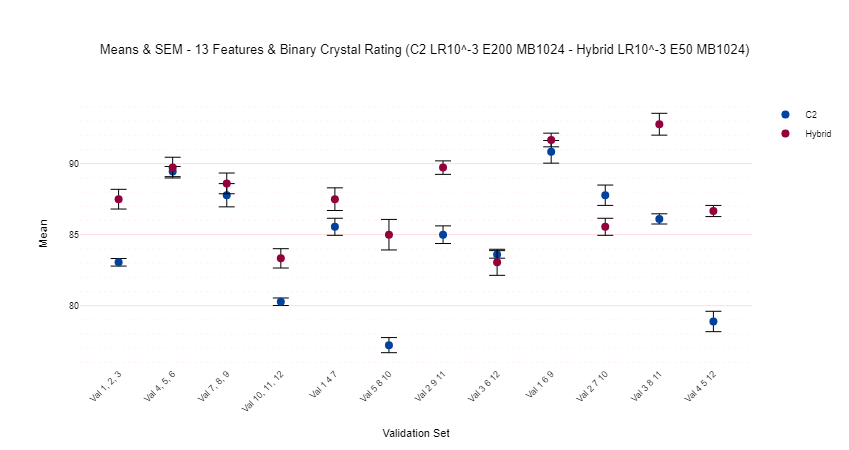
\includegraphics[width=0.8\textwidth]{images/Means & SEM - 13 Features & Binary Crystal Rating (C2 LR10^-3 E200 MB1024 - Hybrid LR10^-3 E50 MB1024).png}
            \end{figure}
        \vspace{0.5cm}
    \item 13 Features \& Continuous Crystal Rating
        \begin{itemize}
        \item Val 2, 7, 10 = C2 (mean = 90.0\%, SEM = 0.79\%), Hybrid (mean = 86.39\%, SEM = 0.73\%)
        \end{itemize}
            \begin{figure}[H]
            \centering
            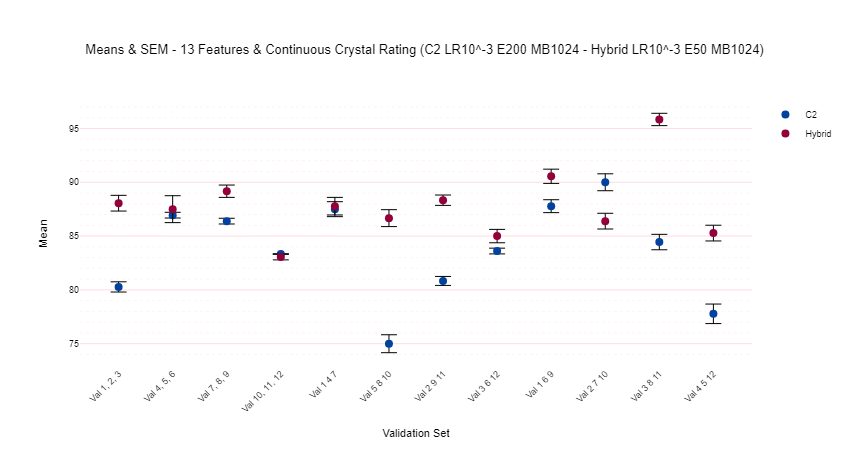
\includegraphics[width=0.8\textwidth]{images/Means & SEM - 13 Features & Continuous Crystal Rating (C2 LR10^-3 E200 MB1024 - Hybrid LR10^-3 E50 MB1024).png}
            \end{figure}
        \vspace{0.5cm}
    \item 12 Features \& Binary Crystal Rating 
        \begin{itemize}
        \item Val 1, 6, 9 = C2 (mean = 89.72\%, SEM = 0.47\%), Hybrid (mean = 89.17\%, SEM = 0.57\%)
        \end{itemize}
            \begin{figure}[H]
            \centering
            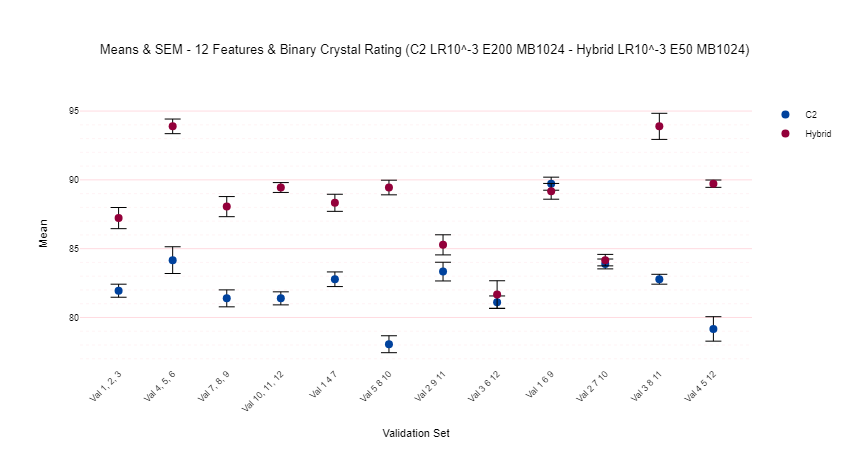
\includegraphics[width=0.8\textwidth]{images/Means & SEM - 12 Features & Binary Crystal Rating (C2 LR10^-3 E200 MB1024 - Hybrid LR10^-3 E50 MB1024).png}
            \end{figure}
        \vspace{0.5cm}
    \item 12 Features \& Continuous Crystal Rating
        \begin{itemize}
        \item Val 3, 6, 12 = C2 (mean = 83.33\%, SEM = 0.39\%), Hybrid (mean = 80.28\%, SEM = 0.83\%)
        \item Val 1, 6, 9 = C2 (mean = 87.50\%, SEM = 0.57\%), Hybrid (mean = 86.67\%, SEM = 0.88\%)
        \end{itemize}
            \begin{figure}[H]
            \centering
            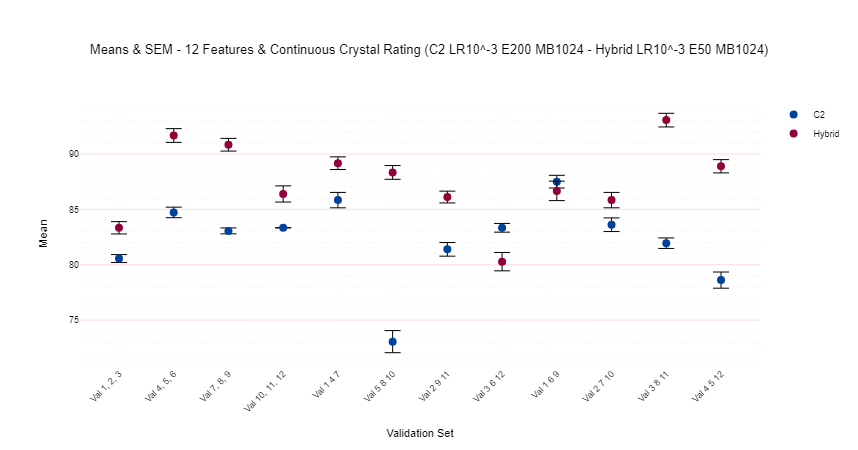
\includegraphics[width=0.8\textwidth]{images/Means & SEM - 12 Features & Continuous Crystal Rating (C2 LR10^-3 E200 MB1024 - Hybrid LR10^-3 E50 MB1024).png}
            \end{figure}
        \vspace{0.5cm}
\end{itemize}
\vspace{0.5cm}

In hindsight I would have have attempted to incorporate ConceptShAP \cite{yehCompletenessawareConceptBasedExplanations2019}, or another method for assessment of concept evaluation.

The increased use case for LLMs is of great intrigue, particularly with the development of multi-modal models, however this will require a far deeper dive by XAI researchers if the outputs are to be worth of trust.
